\documentclass{beamer}
\usepackage{default}
\usetheme{Pittsburgh}
\usecolortheme{seahorse}

\usepackage[brazilian]{babel}

\usepackage{cmap}				% Mapear caracteres especiais no PDF
\usepackage{lmodern}			% Usa a fonte Latin Modern
\usepackage[T1]{fontenc}		% Selecao de codigos de fonte.
\usepackage[utf8]{inputenc}		% Codificacao do documento (conversão automática dos acentos)
\usepackage{indentfirst}		% Indenta o primeiro parágrafo de cada seção.
\usepackage{color}				% Controle das cores
\usepackage{graphicx}			% Inclusão de gráficos
\usepackage{booktabs}           % Pacote para tabelas
\usepackage{pgf,tikz}           % Pacote para o uso do tikz
\usetikzlibrary{arrows}         % Pacote tikz
\usepackage{enumitem}          % Pacote para criação de listas
\usetikzlibrary{matrix,chains,positioning,decorations.pathreplacing,arrows}
\setlist[itemize,1]{label={\fontfamily{cmr}\fontencoding{T1}\selectfont\textbullet}}


\usepackage{amsthm}
\usepackage{amsfonts}
\usepackage{amssymb}
\usepackage{amsmath}
\usepackage{MnSymbol}
\deftranslation[to=brazilian]{Theorem}{Teorema}
\newtheorem{lema}[theorem]{\scshape Lema}
\newtheorem{cor}[theorem]{\scshaé Corol\'ario}
\newtheorem{propo}[theorem]{\scshape Proposi\c{c}\~ao}
\newtheorem{definicao}{\scshape Defini\c{c}\~ao}[section]
\newtheorem{ex}{\scshape Exemplo}[section]
\newtheorem{obs}{Observação}[section]
\usepackage{listings}
\newcommand{\norm}[1]{\left\lVert#1\right\rVert}

\setbeamertemplate{theorems}[numbered]
\usepackage[backend=biber,style=numeric]{biblatex} %oi hehe oi me achou aqui kkk
\addbibresource{ref.bib}
\usepackage{silence,lmodern}
\WarningFilter{biblatex}{Patching footnotes failed}
\usepackage{csquotes}
\usepackage{graphics}
\usepackage{booktabs}
\setbeamertemplate{caption}[numbered]
\usepackage{adjustbox}
\usepackage{listings}


\usepackage{algorithm}
\usepackage{algpseudocode}
\makeatletter
\renewcommand{\ALG@name}{Algoritmo}
\renewcommand{\listalgorithmname}{Lista de algoritmos}
\renewcommand{\algorithmicwhile}{\textbf{enquanto}}
\renewcommand{\algorithmicdo}{\textbf{faça}}
\renewcommand{\algorithmicend}{\textbf{fim}}
\renewcommand{\algorithmicfor}{\textbf{para}}
\newcommand{\INDSTATE}[1][1]{\STATE\hspace{#1\algorithmicindent}}
\definecolor{ttttff}{rgb}{0.2,0.2,1}

\addtobeamertemplate{navigation symbols}{}{%
    \usebeamerfont{footline}%
    \usebeamercolor[fg]{footline}%
    \hspace{1em}%
    \insertframenumber/\inserttotalframenumber
}


\title{Estudo matemático do reconhecimento
de caracteres}
\author[Carlos Ronchi]{Carlos Henrique Venturi Ronchi\\{\small Orientador: Abel Soares Siqueira}}

\institute{Universidade Federal do Paraná - UFPR}

\begin{document}

\begin{frame}
    \titlepage    
\end{frame}

\begin{frame}
    \tableofcontents
\end{frame}

\section{Introdução}
    \begin{frame}{Motivação}
        \begin{itemize}
            \item Prever a inflação;
            \item saber se choverá ou não;
            \item demanda de estoque;
            \item reconhecimento de caracteres.
        \end{itemize}
    \end{frame}
    
    \begin{frame}{Ferramentas}
        \begin{itemize}
            \item Método do gradiente;
            \item método dos gradientes conjugados;
            \item método do gradiente estocástico;
            \item redes neurais;
            \item outros.
        \end{itemize}
    \end{frame}
    
\section{Modelagem}    
    
    \begin{frame}{Funções}
        Para a regressão (e quadrados mínimos), temos
        \begin{equation*}
            J(\theta) = \frac{1}{2} \sum_{i=1}^{m}(y^{(i)}- m_\theta(x^{(i)}))^2.
        \end{equation*}
        
        Já para classificação, 
        \begin{equation*}
            J(\theta) = \sum_{i=1}^{m}\left[-y^{(i)}log(m_\theta(x^{(i)})) - (1-y^{(i)})log(1-m_\theta(x^{(i)}))\right].
        \end{equation*}
    \end{frame}
    
\section{Métodos}
    \subsection{Método do gradiente}
        \begin{frame}{Método do gradiente}
            Direção de descida $-\nabla f(x)$.
            
            \begin{theorem}
                Sejam $f$ uma função convexa e $L$-Lipschitz e $x^{*} \in \arg\min_{x: \norm{x} \leq B} f(x)$. Se rodarmos o método do gradiente em $f$ para $T$ passos com $\eta = \sqrt{\dfrac{B^2}{L^2T}}$, então o vetor de retorno $\bar{x}$ satisfaz 
                \begin{equation*}
                    f(\bar{x}) - f(x^{*}) \leq \frac{BL}{\sqrt{T}}
                \end{equation*}
                Ainda mais, dado $\epsilon > 0$, para obter $f(\bar{x}) - f(x^{*}) \leq \epsilon$, é necesśario rodar o algoritmo com um número $T$ de iterações que satisfaz
                \begin{equation*}
                    T \geq \frac{B^2L^2}{\epsilon^2}.
                \end{equation*}
            \end{theorem}
        \end{frame}

        \begin{frame}{Método do gradiente}
            \begin{figure}
                \centering
                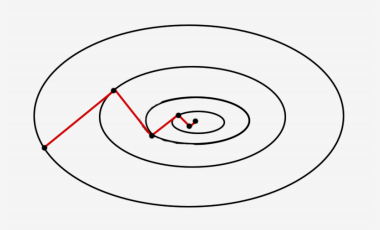
\includegraphics[width=.80\textwidth]{gradiente.png}
                \caption{Passos do método do gradiente}
                \label{fig:gc}
            \end{figure}
        \end{frame}

    \subsection{Método dos gradientes conjugados}
        \begin{frame}{Método dos gradientes conjugados}
            \begin{theorem}
                Seja $f: \mathbb{R}^n \to \mathbb{R}$ e denote por $x^{*}$ seu minimizador global. Então para qualquer $x^0 \in \mathbb{R}^n$, o método das difereções conjugadas gera uma sequência
                \begin{gather*}
                x^{k+1} = x^{k} + t_{k}d^{k} \mbox{, } t_k = \frac{-\nabla f(x^k)^{T}d^k}{(d^k)^{T}Ad^k}\mbox{   } \forall k = 0,...,n-1 ,
                \end{gather*}
                onde $x^n = x^{*}$.
            \end{theorem}
        \end{frame}
        
        \begin{frame}{Método dos gradientes conjugados}
            \begin{figure}
                \centering
                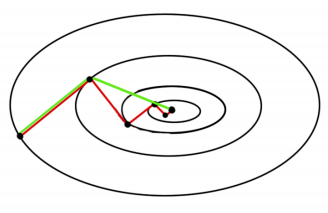
\includegraphics[width=.8\textwidth]{gradienteconj.png}
                \caption{Passos do método dos gradientes conjugados em verde. Em vermelho os passos do método do gradiente}
                \label{fig:my_label}
            \end{figure}    
        \end{frame}
        
    \subsection{Método do gradiente estocástico}
        \begin{frame}{Método do gradiente estocástico}
            Expectativa de um vetor aleatório ser um subgradiente.
            \begin{equation*}
                x^k = x^{k-1} - \alpha d^k\text{, onde }\mathbb{E}[d^k\mbox{ }\vert\mbox{ } x^k] \in \partial f(x^k)
            \end{equation*}
            No caso das funções citadas anteriormente,
            \begin{equation*}
                d^{k} = (m_\theta(x^{(i)}) - y^{(i)})x^{(i)}
            \end{equation*}
        \end{frame}

    \subsection{Redes Neurais}
        \begin{frame}{Redes Neurais}
            \begin{figure}[ht]
            \centering           
            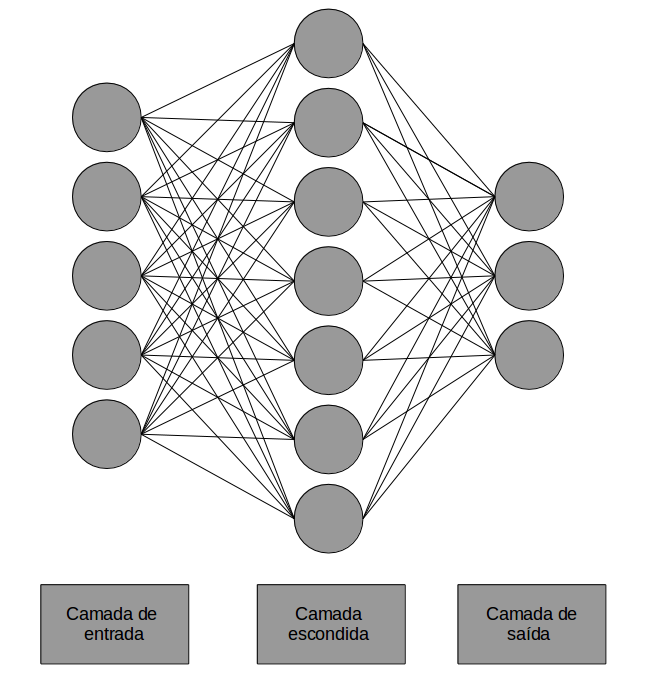
\includegraphics[width=.7\textwidth,height=.7\textheight]{redeneural.png}
            \caption{Esquema de uma rede neural artificial.}
            \label{fig:ann}
            \end{figure}        
        \end{frame}
    
        \begin{frame}{Redes Neurais}
            \begin{itemize}
                \item Backpropagation
                \item Alta capacidade para aprender
                \item Reconhecimento de caracteres
                \item Computação visual em geral
                \item Mercado financeiro
            \end{itemize}
        \end{frame}
\section{Reconhecimento de caracteres}
    \subsection{Testes}
    \begin{frame}{Dados}
        \begin{itemize}
            \item \emph{Detexify}
            \item \emph{Write-math}
            \item \emph{HASYv2 dataset}
            \item $168233$ dados, $369$ classes.
        \end{itemize}
        \begin{figure}
            \centering
            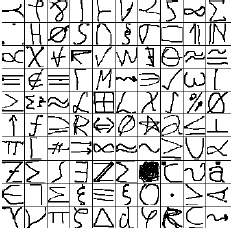
\includegraphics[width=.45\textwidth,height=.45\textheight]{sampleshvsy2.png}
            \caption{Caracteres do banco de dados \emph{HASYv2}}
            \label{fig:samplehasy}
        \end{figure}
    \end{frame}
    
    \begin{frame}{Metodologia}
        \begin{itemize}
            \item TensorFlow
            \item Redes neurais convolucionais
            \item Adam
            \item 10 épocas, batch de tamanho 500
            \item tamanho do passo de $0.0005$
            \item ReLU (ao invés de softmax). 
        \end{itemize}    
    \end{frame}
    
    \begin{frame}{Resultados}
        \begin{figure}[hbt]
            \centering
            
\includegraphics[width=0.5\textwidth]{TesteUFPR.png}
            \caption{Imagem utilizada para teste prático do modelo.}
            \label{fig:parufpr}
        \end{figure}
        
         \begin{table}[htb]
            \centering
            \caption{Letras reconhecidas da Figura \ref{fig:parufpr} pelo modelo.}
            \label{tab:parufpr}
            \begin{tabular}{@{}clllll@{}}
                \toprule
                \textbf{Letra Original}    & \multicolumn{1}{c}{$\partial$} & \multicolumn{1}{c}{U} &     \multicolumn{1}{c}{F} & \multicolumn{1}{c}{P} & \multicolumn{1}{c}{R} \\ \midrule
                \textbf{Letra reconhecida} & $\partial$                     & $\cup$                & F                     & $\nabla$              & $\mathcal{R}$         \\ \bottomrule
            \end{tabular}
        \end{table}
    \end{frame}
    
    \begin{frame}
        \begin{figure}[htb]
            \centering
            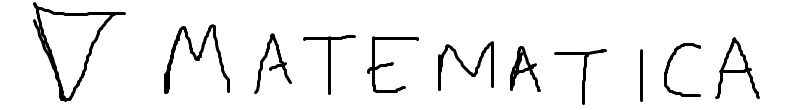
\includegraphics[width=0.9\textwidth]{TesteMat.png}
            \caption{Imagem para utilizar no teste do programa.}
            \label{fig:nabmat}
        \end{figure}
        
        \begin{table}[htb]
            \centering
            \caption{Letras reconhecidas da Figura \ref{fig:nabmat} pelo modelo.}
            \label{tab:nabmat}
            \begin{adjustbox}{max width=\textwidth}
            \begin{tabular}{@{}lccccccccccc@{}}
                \toprule
                \textbf{Letra Original}    & $\nabla$ & M & A        & T      & E     & M & A         & T      & I    & C         & A \\ \midrule
                \textbf{Letra reconhecida} & $\nabla$ & M & $\Delta$ & $\top$ & $\in$ & M & $\lambda$ & $\top$ & $\&$ & $\subset$ & A \\ \bottomrule
            \end{tabular}
            \end{adjustbox}
        \end{table}
    \end{frame}
    
    \begin{frame}{Próximos passos}
        \begin{itemize}
            \item Segmentação de caracteres
            \item Desenvolvimento de modelos \emph{state-of-the-art}
            \item Código no Github
        \end{itemize}
    \end{frame}
    
\section{Referências}
    \begin{frame}[allowframebreaks]{Referências}
        \nocite{thomadata,tensorflow2015,zhang,elzad,nocedal,shai, ng,mitchell,wfan,julia,github,burfa,adam,bajmes,tensorflow2015}
        \printbibliography[heading=none]
    \end{frame}
    
   
\end{document}
